\capitulo{1}{Introducción}

Gracias al avance de las técnicas y algoritmos de minería de datos, disciplinas no directamente relacionadas con la computación se han ido beneficiando de las ciencias de datos, a modo particular, la medicina está desarrollándose hacia modelos más preventivos gracias a las predicciones que se pueden generar utilizando estos métodos.

Es por este motivo que podemos ver en la literatura científica de los últimos años como se relaciona medicina y ciencia de datos, por ejemplo en estudios de detección de caídas~\cite{tolkiehn2011fall} o la motorización del sueño para la prevención de apneas~\cite{kortelainen2012sleepmonitoring}. En este trabajo de fin de grado, el objetivo es la detección de crisis epilépticas a partir de sensores de presión en un colchón y constantes vitales del paciente. Este TFG está adscrito al proyecto homónimo vencedor del concurso universitario \textit{Desafío Universidad Empresa}~\cite{radio:radio_amiga_burgos_2018}

\begin{table}
	\centering
	\resizebox{\textwidth}{!}
	{\begin{tabular}{|lccr|}
			\hline 
			\textbf{Hardware} & \textbf{Coste} & \textbf{Fiabilidad} & \textbf{Observación} \\ 
			\hline 
			Detector de EEG & Elevado & Elevada & Incómodo para dormir \\ 
			\hline 
			Pulseras inteligentes & Bajo & Elevada & Los pacientes son propensos a quitársela \\ 
			\hline 
			Cama inteligente & Elevado & Pendiente de estudio & Es cómodo y no invasivo \\ 
			\hline 
	\end{tabular}}
	\caption{Distintos métodos para la detección de crisis epilépticas y sus situaciones según \textit{PRONISA}.}
	\label{tab:modelos}
\end{table}

\begin{figure}
	\centering
	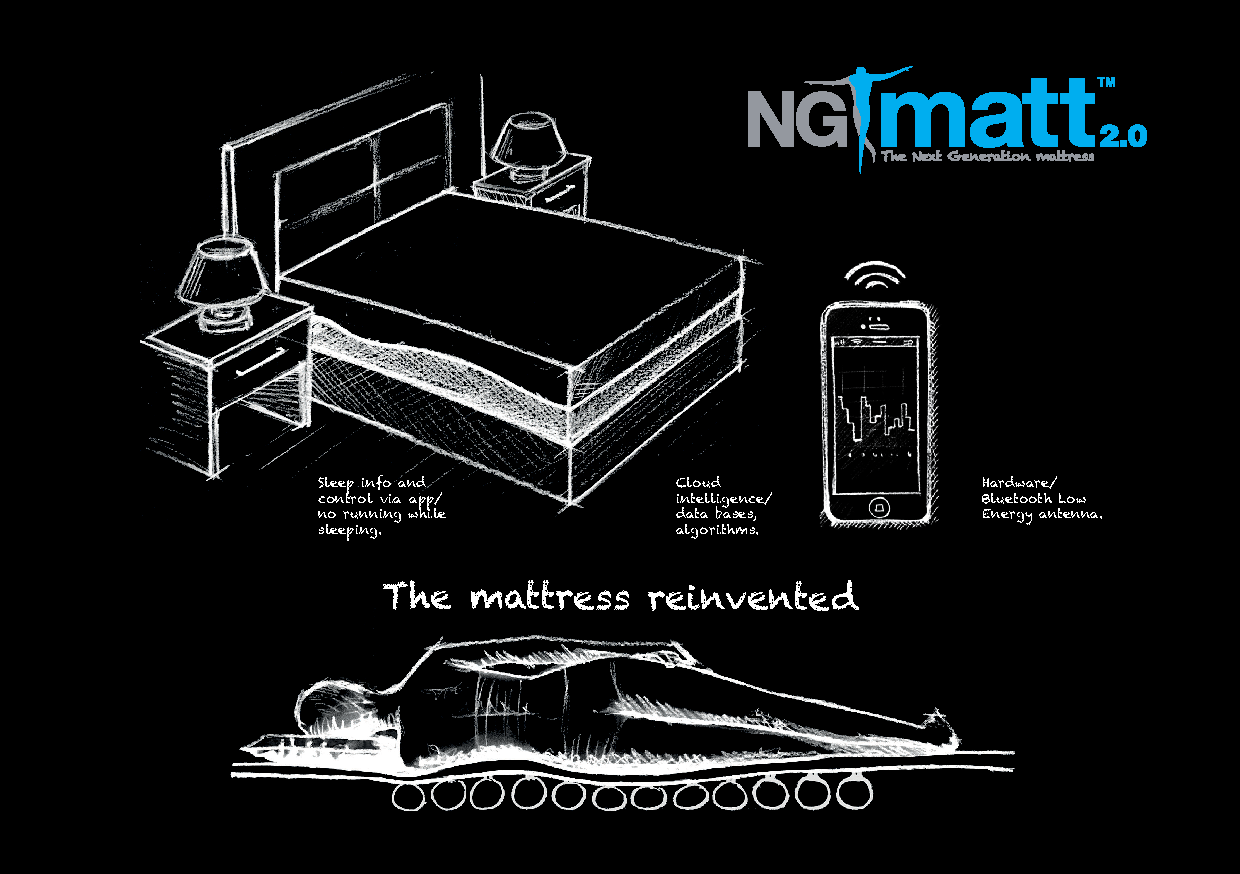
\includegraphics[width=\textwidth]{cama_publicidad}
	\caption{Publicidad de la cama de la cual obtenemos los datos.}
	\label{fig:cama_publi}
\end{figure}

Aunque el análisis y detección de crisis epilépticas de manera automática ha sido ampliamente explorada por la comunidad científica, esta se ha centrado o en el uso de pulseras inteligentes~\cite{ramgopal2014product_review} o el uso de encefalogramas~(\textit{EEG})~\cite{jeppesen2017modified,kumar2014epilepticeeg,tzallas2012review} para la predicción de estos eventos. Por tanto, ante pacientes con diversos problemas de salud que impiden el uso de pulseras ya que son fácilmente removibles y de dispositivos de control de actividad cerebral al entorpecer el sueño del paciente (Tabla~\ref{tab:modelos}), se realiza este proyecto que enfoca la detección de las crisis epilépticas en el uso de sensores de presión y biométricos en la cama (Fig.~\ref{fig:cama_publi} donde duerme el paciente. 



\section{Material adjunto}
Junto a esta memoria se incluyen:

\begin{itemize}
	\item \textbf{Cuaderno de investigación} con la evolución y pasos realizados durante la investigación junto con los resultados de cada experimento.
	\item \textbf{Anexos} donde se incluyen:
		\begin{itemize}
			\item Plan de proyectos
			\item Requisitos del sistema
			\item Diseño del sistema
			\item Manual para el programador
			\item Manual para el usuario
		\end{itemize}
	\item \textbf{API REST} en \textbf{Python-Flask}
	\item \textbf{Aplicación web} que funciona sobre la \textit{API}.
	\item \textbf{Experimentos} en \textit{Jupyter Notebook}
\end{itemize}

Además se puede acceder a través de internet a la \href{https://ubu.joselucross.com}{ página web en producción} y al \href{https://github.com/jlgarridol/TFG-Smartbeds}{repositorio GitHub del proyecto}.